\section{Proof of theorem \ref{teoFlex}}\label{secTeoFlex}

In this section, we shall prove theorem \ref{teoFlex}. For $o=[n]$, the result holds because for any translation in the plane, the compactification  $f$  verifies $o(f)=[n]$. For this type of maps, all the mutually singular sets consist of a single set and by theorem \ref{TeoCod}, we conclude the existence of a map such that $o(f)=[n]$. 

Now, we are only interested in the case $[n^2]\leq o \leq \sup(\Pol)$. First, we are going to prove the result for the particular case $o\in \L$, and then, adapt to obtain the general result ($o\in\CL$).


\subsection{Construction of the map}

We are going to recall the construction done in \cite{HaRo19} that will provide us a homeomorphism $f:S^2\to S^2$. Let us fix $[a(n)]\in \L$ such that $[n^2]< [a(n)]< \sup(\Pol)$. For said  $[a(n)]$, there must exist $L\geq 3$ such that $[a(n)]\leq [n^L]$. From now on, $L$ is going to be fixed. 

Let us consider $P_1,\cdots, P_{L+2}$ copies of the plane $\R^2$. For each $P_i$ we denote $O_i=\{(x,y)\in P_i: y>0\}$ the upper half plane. For each $i=1,\cdots, L+1$ we are going to select maps $\varphi_i:(0,\infty)\to \R$ and with them, define $\Phi_i:O_i\to O_{i+1}$ by
$\Phi_i(x,y)=(x+\varphi_i(y),y)$.

The first property we want for $\varphi_i$ is the limit in $0$ be $-\infty$. Now, we define $\sim$ the equivalence relation in $\cup P_i$ generated by $(x,y)\sim \Phi_i(x,y)$ if $(x,y)\in O_i$. The quotient space $P=\cup P_i/\sim$  is a Hausdorff simply connected non-compact surface, and thus is homeomorphic to the plane. Figure \ref{imgPlaneP} represents the quotient space $P$.  


\begin{figure}[h!]
\begin{center}


\tikzset{every picture/.style={line width=0.75pt}} %set default line width to 0.75pt        

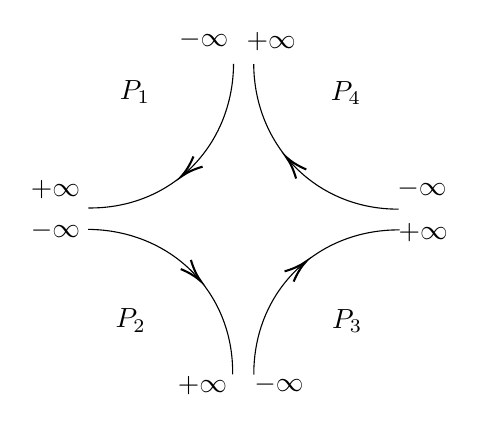
\begin{tikzpicture}[x=0.75pt,y=0.75pt,yscale=-1,xscale=1]
%uncomment if require: \path (0,300); %set diagram left start at 0, and has height of 300

%Curve Lines [id:da8105529734511654] 
\draw    (190.36,109.77) .. controls (230.21,110.23) and (260.07,79.97) .. (260.35,40.33) ;
\draw [shift={(235.08,94.69)}, rotate = 318.25] [color={rgb, 255:red, 0; green, 0; blue, 0 }  ][line width=0.75]    (10.93,-3.29) .. controls (6.95,-1.4) and (3.31,-0.3) .. (0,0) .. controls (3.31,0.3) and (6.95,1.4) .. (10.93,3.29)   ;
%Curve Lines [id:da5656492723103168] 
\draw    (270.06,40.44) .. controls (270.33,80.11) and (300.56,110.56) .. (339.89,110.33) ;
\draw [shift={(285.7,85.21)}, rotate = 48.47] [color={rgb, 255:red, 0; green, 0; blue, 0 }  ][line width=0.75]    (10.93,-3.29) .. controls (6.95,-1.4) and (3.31,-0.3) .. (0,0) .. controls (3.31,0.3) and (6.95,1.4) .. (10.93,3.29)   ;
%Curve Lines [id:da12429852092804805] 
\draw    (340.33,120.33) .. controls (300.33,120.11) and (269.92,150.08) .. (270.11,190.11) ;
\draw [shift={(295.31,135.52)}, rotate = 138.47] [color={rgb, 255:red, 0; green, 0; blue, 0 }  ][line width=0.75]    (10.93,-3.29) .. controls (6.95,-1.4) and (3.31,-0.3) .. (0,0) .. controls (3.31,0.3) and (6.95,1.4) .. (10.93,3.29)   ;
%Curve Lines [id:da13626418538311813] 
\draw    (259.92,189.92) .. controls (260.38,149.77) and (229.62,120.38) .. (190.23,120.08) ;
\draw [shift={(244.66,145.14)}, rotate = 228.09] [color={rgb, 255:red, 0; green, 0; blue, 0 }  ][line width=0.75]    (10.93,-3.29) .. controls (6.95,-1.4) and (3.31,-0.3) .. (0,0) .. controls (3.31,0.3) and (6.95,1.4) .. (10.93,3.29)   ;

% Text Node
\draw (204.29,47.17) node [anchor=north west][inner sep=0.75pt]    {$P_{1}$};
% Text Node
\draw (202.29,157.17) node [anchor=north west][inner sep=0.75pt]    {$P_{2}$};
% Text Node
\draw (306.57,157.26) node [anchor=north west][inner sep=0.75pt]    {$P_{3}$};
% Text Node
\draw (306,47.46) node [anchor=north west][inner sep=0.75pt]    {$P_{4}$};
% Text Node
\draw (232.86,23.17) node [anchor=north west][inner sep=0.75pt]    {$-\infty $};
% Text Node
\draw (265.43,24.03) node [anchor=north west][inner sep=0.75pt]    {$+\infty $};
% Text Node
\draw (161.43,114.97) node [anchor=north west][inner sep=0.75pt]    {$-\infty $};
% Text Node
\draw (269.14,189.26) node [anchor=north west][inner sep=0.75pt]    {$-\infty $};
% Text Node
\draw (338,94.6) node [anchor=north west][inner sep=0.75pt]    {$-\infty $};
% Text Node
\draw (338.57,115.83) node [anchor=north west][inner sep=0.75pt]    {$+\infty $};
% Text Node
\draw (232.29,189.54) node [anchor=north west][inner sep=0.75pt]    {$+\infty $};
% Text Node
\draw (161.43,94.97) node [anchor=north west][inner sep=0.75pt]    {$+\infty $};


\end{tikzpicture}
\caption{Gluing of the plane $P$ for $L=3$.} \label{imgPlaneP}
\end{center} 
\end{figure}


Let $T:\cup P_i\to \cup P_i$ be defined as the translation $T(x,y)=(x+1,y)$ on each $P_i$.  The map $T$ commutes with each $\Phi_i$ and therefore it defines $F:P\to P$ as an orientation preserving homeomorphism on the plane without fixed points. The map $F$ induces a homeomorphism $f$ in the compactification of the plane $\R^2\cup \{\infty\}= S^2$, which verifies $\Omega(f)=\{\infty\}$. In particular, we can apply theorem  \ref{TeoCod} to compute its generalized entropy. Figure \ref{imgMapf} represents the dynamics of $f$.

\begin{figure}[h!]
\begin{center}


\tikzset{every picture/.style={line width=0.75pt}} %set default line width to 0.75pt        

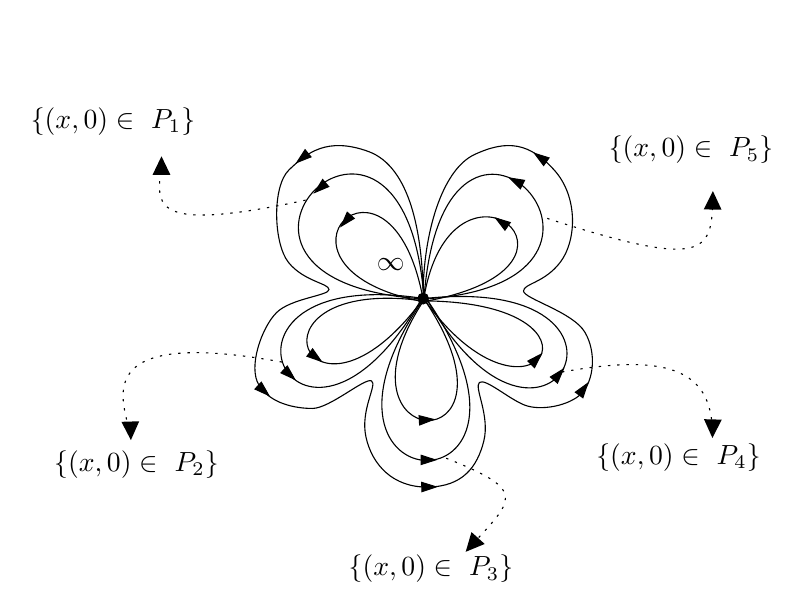
\begin{tikzpicture}[x=0.75pt,y=0.75pt,yscale=-1,xscale=1]
%uncomment if require: \path (0,300); %set diagram left start at 0, and has height of 300

%Curve Lines [id:da30518124245165645] 
\draw    (299.4,141.74) .. controls (244,215.5) and (209.1,128.99) .. (300.34,141.53) ;
%Curve Lines [id:da8950808475599585] 
\draw    (300.34,141.53) .. controls (397.67,142.17) and (352.67,212.5) .. (301.28,141.61) ;
%Shape: Circle [id:dp7083342407214686] 
\draw  [fill={rgb, 255:red, 0; green, 0; blue, 0 }  ,fill opacity=1 ] (297.63,140.42) .. controls (297.63,138.99) and (298.78,137.84) .. (300.21,137.84) .. controls (301.63,137.84) and (302.79,138.99) .. (302.79,140.42) .. controls (302.79,141.84) and (301.63,143) .. (300.21,143) .. controls (298.78,143) and (297.63,141.84) .. (297.63,140.42) -- cycle ;
%Curve Lines [id:da9719941367446978] 
\draw    (298.03,140.42) .. controls (171,131) and (291.07,10.17) .. (300.61,140.42) ;
%Curve Lines [id:da38242804392902285] 
\draw    (300.61,140.42) .. controls (310.2,10.2) and (423.11,131.57) .. (303.19,140.42) ;
%Curve Lines [id:da569057900625008] 
\draw    (300.61,140.42) .. controls (419.97,127.57) and (359.97,243.29) .. (301.82,140.54) ;
%Curve Lines [id:da0472317528556514] 
\draw    (299.4,140.72) .. controls (238.6,245) and (183,122.2) .. (300.61,140.42) ;
%Curve Lines [id:da2970606376255487] 
\draw    (300.21,137.84) .. controls (299.75,109.81) and (294.2,77) .. (273.86,69.57) .. controls (253.51,62.14) and (243.8,70.6) .. (235.57,78.43) .. controls (227.34,86.26) and (228.04,113.98) .. (235.38,123.06) .. controls (242.71,132.14) and (254.88,133.13) .. (254.86,136.07) .. controls (254.84,139.01) and (236.57,140.26) .. (229.57,147.19) .. controls (222.57,154.12) and (215.66,173.26) .. (221.1,182.14) .. controls (226.53,191.03) and (238.57,193.36) .. (246.86,193.36) .. controls (255.14,193.36) and (272.14,178.43) .. (275.29,180.07) .. controls (278.43,181.71) and (269.76,193.98) .. (272.67,207.17) .. controls (275.57,220.36) and (285.51,231.43) .. (302.41,231.24) .. controls (319.32,231.04) and (326.32,221.45) .. (329.43,209.07) .. controls (332.54,196.69) and (324.52,183.02) .. (327.33,180.83) .. controls (330.14,178.64) and (341.46,188.77) .. (349.09,191.74) .. controls (356.71,194.71) and (370.71,192.14) .. (376.57,186.07) .. controls (382.43,180) and (383.86,166.43) .. (378.14,156.64) .. controls (372.43,146.86) and (348.57,140.41) .. (348.57,136.79) .. controls (348.57,133.16) and (358.71,133) .. (366.43,122.71) .. controls (374.14,112.43) and (375,91.29) .. (363.29,78.43) .. controls (351.57,65.57) and (341,63.57) .. (325,71) .. controls (309,78.43) and (300.38,109.69) .. (300.21,137.84) -- cycle ;
%Curve Lines [id:da4196238518994797] 
\draw  [dash pattern={on 0.84pt off 2.51pt}]  (360,101.8) .. controls (436.62,126.5) and (439.3,118.43) .. (439.76,91.59) ;
\draw [shift={(439.8,88.6)}, rotate = 90.78] [fill={rgb, 255:red, 0; green, 0; blue, 0 }  ][line width=0.08]  [draw opacity=0] (8.93,-4.29) -- (0,0) -- (8.93,4.29) -- cycle    ;
%Curve Lines [id:da512673420318001] 
\draw  [dash pattern={on 0.84pt off 2.51pt}]  (311.31,217.34) .. controls (351.12,233.17) and (343.97,236.82) .. (322.4,260.56) ;
\draw [shift={(320.71,262.43)}, rotate = 311.95] [fill={rgb, 255:red, 0; green, 0; blue, 0 }  ][line width=0.08]  [draw opacity=0] (8.93,-4.29) -- (0,0) -- (8.93,4.29) -- cycle    ;
%Curve Lines [id:da8363660989464397] 
\draw  [dash pattern={on 0.84pt off 2.51pt}]  (232.14,171) .. controls (137.89,153.8) and (155.95,190.09) .. (159.02,205.68) ;
\draw [shift={(159.4,208.6)}, rotate = 268.26] [fill={rgb, 255:red, 0; green, 0; blue, 0 }  ][line width=0.08]  [draw opacity=0] (8.93,-4.29) -- (0,0) -- (8.93,4.29) -- cycle    ;
%Curve Lines [id:da1537579559441531] 
\draw  [dash pattern={on 0.84pt off 2.51pt}]  (243.57,93) .. controls (163.77,110.1) and (172.93,93.68) .. (174.05,74.85) ;
\draw [shift={(174.14,71.86)}, rotate = 90] [fill={rgb, 255:red, 0; green, 0; blue, 0 }  ][line width=0.08]  [draw opacity=0] (8.93,-4.29) -- (0,0) -- (8.93,4.29) -- cycle    ;
%Shape: Triangle [id:dp8958619795940812] 
\draw  [fill={rgb, 255:red, 0; green, 0; blue, 0 }  ,fill opacity=1 ] (239.39,74.83) -- (243.32,68.72) -- (246.14,72.16) -- cycle ;
%Shape: Triangle [id:dp7323275141016883] 
\draw  [fill={rgb, 255:red, 0; green, 0; blue, 0 }  ,fill opacity=1 ] (247.99,89.28) -- (251.78,83.09) -- (254.69,86.47) -- cycle ;
%Shape: Triangle [id:dp5439908412868601] 
\draw  [fill={rgb, 255:red, 0; green, 0; blue, 0 }  ,fill opacity=1 ] (260.74,105.52) -- (263.63,98.86) -- (266.98,101.8) -- cycle ;
%Shape: Triangle [id:dp6482573513096812] 
\draw  [fill={rgb, 255:red, 0; green, 0; blue, 0 }  ,fill opacity=1 ] (225.83,187.05) -- (219.23,184.03) -- (222.24,180.74) -- cycle ;
%Shape: Triangle [id:dp3538986571399132] 
\draw  [fill={rgb, 255:red, 0; green, 0; blue, 0 }  ,fill opacity=1 ] (238.31,179.28) -- (231.73,176.21) -- (234.76,172.95) -- cycle ;
%Shape: Triangle [id:dp3410795032956404] 
\draw  [fill={rgb, 255:red, 0; green, 0; blue, 0 }  ,fill opacity=1 ] (251.11,170.61) -- (244.26,168.23) -- (246.94,164.67) -- cycle ;
%Shape: Triangle [id:dp4803111514559295] 
\draw  [fill={rgb, 255:red, 0; green, 0; blue, 0 }  ,fill opacity=1 ] (379.46,181.28) -- (377.17,188.17) -- (373.57,185.53) -- cycle ;
%Shape: Triangle [id:dp3708997709224997] 
\draw  [fill={rgb, 255:red, 0; green, 0; blue, 0 }  ,fill opacity=1 ] (367.75,174.42) -- (364.93,181.11) -- (361.55,178.2) -- cycle ;
%Shape: Triangle [id:dp975132604650822] 
\draw  [fill={rgb, 255:red, 0; green, 0; blue, 0 }  ,fill opacity=1 ] (357.14,167.17) -- (353.87,173.65) -- (350.7,170.52) -- cycle ;
%Shape: Triangle [id:dp41553716907224714] 
\draw  [fill={rgb, 255:red, 0; green, 0; blue, 0 }  ,fill opacity=1 ] (335.21,101.69) -- (342.16,103.78) -- (339.62,107.45) -- cycle ;
%Shape: Triangle [id:dp7180277186575779] 
\draw  [fill={rgb, 255:red, 0; green, 0; blue, 0 }  ,fill opacity=1 ] (341.89,82.35) -- (349.06,83.47) -- (347.06,87.45) -- cycle ;
%Shape: Triangle [id:dp33809986896433] 
\draw  [fill={rgb, 255:red, 0; green, 0; blue, 0 }  ,fill opacity=1 ] (353.9,70.48) -- (360.83,72.65) -- (358.26,76.29) -- cycle ;
%Curve Lines [id:da32436656754150617] 
\draw    (301.82,140.54) .. controls (374.2,245.8) and (229.4,243) .. (300.61,140.42) ;
%Curve Lines [id:da8523403673333396] 
\draw    (298.34,141.53) .. controls (215,124.5) and (284.67,54.83) .. (300.34,141.53) ;
%Curve Lines [id:da3938486210267571] 
\draw    (300.34,141.53) .. controls (313,59.83) and (394.67,124.17) .. (302.34,141.53) ;
%Curve Lines [id:da34419357175849075] 
\draw    (301.28,141.61) .. controls (353.67,220.5) and (251.67,216.17) .. (300.34,141.53) ;
%Curve Lines [id:da15164910719694302] 
\draw  [dash pattern={on 0.84pt off 2.51pt}]  (367.14,175.8) .. controls (416.34,166.99) and (439.05,173.71) .. (439.59,204.63) ;
\draw [shift={(439.57,207.57)}, rotate = 271.47] [fill={rgb, 255:red, 0; green, 0; blue, 0 }  ][line width=0.08]  [draw opacity=0] (8.93,-4.29) -- (0,0) -- (8.93,4.29) -- cycle    ;
%Shape: Triangle [id:dp881720647037963] 
\draw  [fill={rgb, 255:red, 0; green, 0; blue, 0 }  ,fill opacity=1 ] (306.11,218.16) -- (299.2,220.38) -- (299.2,215.92) -- cycle ;
%Shape: Triangle [id:dp30862525793679474] 
\draw  [fill={rgb, 255:red, 0; green, 0; blue, 0 }  ,fill opacity=1 ] (306.47,231.14) -- (299.59,233.46) -- (299.54,229) -- cycle ;
%Shape: Triangle [id:dp6612684939262838] 
\draw  [fill={rgb, 255:red, 0; green, 0; blue, 0 }  ,fill opacity=1 ] (305.28,198.67) -- (298.52,201.3) -- (298.25,196.86) -- cycle ;

% Text Node
\draw (276.69,119.97) node [anchor=north west][inner sep=0.75pt]    {$\infty $};
% Text Node
\draw (109.94,47.09) node [anchor=north west][inner sep=0.75pt]    {$\{( x,0) \in \ P_{1}\}$};
% Text Node
\draw (388.4,60.92) node [anchor=north west][inner sep=0.75pt]    {$\{( x,0) \in \ P_{5}\}$};
% Text Node
\draw (121.2,212.4) node [anchor=north west][inner sep=0.75pt]    {$\{( x,0) \in \ P_{2}\}$};
% Text Node
\draw (263.09,262.8) node [anchor=north west][inner sep=0.75pt]    {$\{( x,0) \in \ P_{3}\}$};
% Text Node
\draw (382.4,209.2) node [anchor=north west][inner sep=0.75pt]    {$\{( x,0) \in \ P_{4}\}$};


\end{tikzpicture}
\caption{ Dynamics of $f$ for $L=3$.} \label{imgMapf}
\end{center} 
\end{figure}

To compute $o(f)$, we need first to understand the location of the mutually singular sets. Let us call $\pi:\cup P_i\to P$ the projection and for each $i$, define $Y_i=\pi([-1/3,1/3]\times [0,1])$ with $[-1/3,1/3]\times [0,1]\subset P_i$. For the map constructed $f$, the family of sets $\{Y_1,\cdots, Y_{L+2}\}$ is mutually singular. Moreover, any other family of mutually singular sets, up to iteration of its elements with a diameter small enough, is equivalent to this one.  Figure \ref{imgMutSingLoc} represents the location of the sets $Y_i$.


\begin{figure}[h!]
\begin{center}


\tikzset{every picture/.style={line width=0.75pt}} %set default line width to 0.75pt        

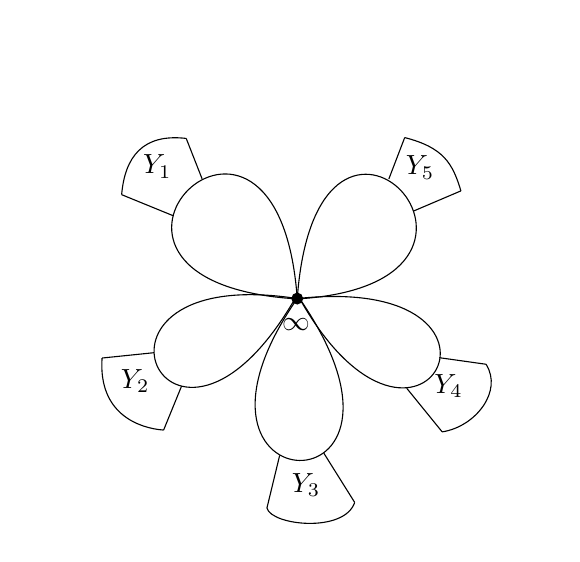
\begin{tikzpicture}[x=0.75pt,y=0.75pt,yscale=-1,xscale=1]
%uncomment if require: \path (0,300); %set diagram left start at 0, and has height of 300

%Shape: Circle [id:dp7083342407214686] 
\draw  [fill={rgb, 255:red, 0; green, 0; blue, 0 }  ,fill opacity=1 ] (318.03,160.42) .. controls (318.03,158.99) and (319.18,157.84) .. (320.61,157.84) .. controls (322.03,157.84) and (323.19,158.99) .. (323.19,160.42) .. controls (323.19,161.84) and (322.03,163) .. (320.61,163) .. controls (319.18,163) and (318.03,161.84) .. (318.03,160.42) -- cycle ;
%Straight Lines [id:da19414039517098103] 
\draw    (236,110.36) -- (260.8,120.49) ;
%Straight Lines [id:da29971771451796636] 
\draw    (267.12,83.27) -- (274.76,102.72) ;
%Curve Lines [id:da7435259387728064] 
\draw    (236,110.36) .. controls (237.57,92.21) and (246.14,80.79) .. (267.12,83.27) ;
%Straight Lines [id:da07101586930277581] 
\draw    (373.37,203.64) -- (390.43,224.64) ;
%Straight Lines [id:da7917861878268071] 
\draw    (411.57,192.07) -- (389.04,188.9) ;
%Curve Lines [id:da4133342138016929] 
\draw    (390.43,224.64) .. controls (406.43,222.21) and (419.86,205.07) .. (411.57,192.07) ;
%Straight Lines [id:da5383846402802042] 
\draw    (306,261.36) -- (312.14,235.97) ;
%Straight Lines [id:da8518330838747479] 
\draw    (348.29,258.64) -- (333.43,234.93) ;
%Curve Lines [id:da23566728066124498] 
\draw    (306,261.36) .. controls (308.29,269.79) and (343.29,273.5) .. (348.29,258.64) ;
%Straight Lines [id:da762381646340947] 
\draw    (264.86,202.64) -- (256.22,223.78) ;
%Straight Lines [id:da9039571065100749] 
\draw    (251.57,186.5) -- (226.57,189.07) ;
%Curve Lines [id:da7565934536737868] 
\draw    (256.22,223.78) .. controls (244.44,222.89) and (224.71,216.07) .. (226.57,189.07) ;
%Curve Lines [id:da13749673732521273] 
\draw    (318.03,160.42) .. controls (191,151) and (311.07,30.17) .. (320.61,160.42) ;
%Curve Lines [id:da042927389844338304] 
\draw    (320.61,160.42) .. controls (330.2,30.2) and (443.11,151.57) .. (323.19,160.42) ;
%Curve Lines [id:da05651797713713891] 
\draw    (320.61,160.42) .. controls (439.97,147.57) and (379.97,263.29) .. (321.82,160.54) ;
%Curve Lines [id:da7966979516183663] 
\draw    (319.4,160.72) .. controls (258.6,265) and (203,142.2) .. (320.61,160.42) ;
%Curve Lines [id:da9750553649479012] 
\draw    (321.82,160.54) .. controls (394.2,265.8) and (249.4,263) .. (320.61,160.42) ;
%Straight Lines [id:da2128761647975621] 
\draw    (376.7,118.23) -- (399.46,108.54) ;
%Straight Lines [id:da6681942399159944] 
\draw    (372.38,82.85) -- (364.75,102.78) ;
%Curve Lines [id:da24887927005881938] 
\draw    (399.46,108.54) .. controls (395.46,95.15) and (391,87.62) .. (372.38,82.85) ;

% Text Node
\draw (312.02,168.97) node [anchor=north west][inner sep=0.75pt]    {$\infty $};
% Text Node
\draw (245.1,90) node [anchor=north west][inner sep=0.75pt]    {$Y_{1}$};
% Text Node
\draw (385.39,195.92) node [anchor=north west][inner sep=0.75pt]    {$Y_{4}$};
% Text Node
\draw (316.7,243.4) node [anchor=north west][inner sep=0.75pt]    {$Y_{3}$};
% Text Node
\draw (234.42,193.2) node [anchor=north west][inner sep=0.75pt]    {$Y_{2}$};
% Text Node
\draw (371.63,90.49) node [anchor=north west][inner sep=0.75pt]    {$Y_{5}$};


\end{tikzpicture}
\caption{ Locations of sets $Y_i$ for $L=3$.} \label{imgMutSingLoc}
\end{center} 
\end{figure}



 The key observation to be made is that for a point $(x,y)\in P_i$ such that its projection $\pi(x,y)\in Y_i$ needs for $-\varphi_i(y)>0$ iterates to reach $Y_{i+1}$. This means, that with the height $y$, we can control the amount of time the point $\pi(x,y)\in Y_1$ is going to need to reach each one of the sets $Y_i$.   


\subsection{Proof of the theorem for the particular case} \label{secPartCase}

Up to this point, we have followed the construction done \cite{HaRo19}. Our next step will be to modify the choice of the maps $\f_i$  done in \cite{HaRo19} such that $[c_{f,\F}(n)]=[a(n)]$.

Let us construct $\varphi_i$ by steps. We shall chose $\f_1$ such that it is negative, increasing, and, for each positive integer $k_1$, assumes the value $-k_1$ on a non trivial interval $I_{k_1}$. This collection of intervals tends to $0$ when $k_1$ tends to $+\infty$. For convenience, we assume that all these intervals are included in the interval $\left. (0, 1 \right]$. The number $k_1$ is going to be our main variable, and we would like to stress that any point of the form $\pi(x,y)\in Y_1$ with $y\in I_{k_1}$ is going to need $k_1$ iterates of $f$ to reach $Y_2$.

Now we look at $k_1$ iterations of the points in the previous step that are in $Y_2$. These points do have the same height $y$ when looked in $P_2$.  The restriction of $\f_2$ to $I_{k_1}$ tell us how many iterates are needed for these points in $Y_2$ to reach $Y_3$. We are going to ask that $\f_2$ restricted to $I_{k_1}$ is continuous, increasing and varies from $-(k_1+a_2(k_1))$ to $-k_1$ (we postpone for later the choice of the integer $0< a_2(k_1)\leq k_1$). Moreover, we need that for each integer $-k_2$ in the interval  $[-(k_1+ a_2(k_1)),-k_1]$, $\f_2$ assumes the value $-k_2$ on a non trivial sub-interval $I_{k_1,k_2}\subset I_{k_1}$.  Now, any point with height in  $I_{k_1,k_2}$ is going to need $k_1$ iterations to go from $Y_1$ to $Y_2$ and $k_2$ iterations to go from $Y_2$ to $Y_3$. We would like to observe that for fixed $k_1$, there are $a_2(k_1)$ possible iterations needed to reach from $Y_2$ to $Y_3$. Finally, we would like remark that we chose the interval $[-(k_1+ a_2(k_1)),-k_1]$ instead of $[-a_2(k_1),0]$ because we also need that the limit of $\f_2$ in $0$ be $-\infty$.  

Likewise, we define $\f_3$ to be increasing on each interval $I_{k_1,k_2}$ and assume each integer $-k_3$ between $-(3k_1-k_2+a_3(k_1))$ and $-(3k_1-k_2)$ on a non trivial sub-interval $I_{k_1,k_2,k_3}$ of $I_{k_1,k_2}$. To explain why we choose the interval like this, first observe that $2k_1 \leq k_1+ k_2 \leq 3k_1$. By the choice of the interval, if $0< a_3(k_1)\leq k_1$, then,
\[4k_1 \leq k_1+k_2+k_3 \leq 5k_1.\]
This gives us the following control: A point in $Y_1$ with height in $I_{k_1}$ is going to reach $Y_2$ in $k_1$ iterates, reach $Y_3$ in between $2k_1$ to $3k_1$ iterates and $Y_4$ in between $4k_1$ to $5k_1$ iterates. Similar to the previous step, for $k_1$ fixed, there are $a_3(k_1)$ possible iterations needed to reach from $Y_3$ to $Y_4$. 
	
We define $\f_i$ inductively until $\f_{L+1}$. The map $\f_{i+1}$ is chosen such that for $k_1, \cdots, k_i$ fixed, it assumes each integer value $-k_{i+1}$ in a sub-interval $I_{k_1,\cdots,k_{i+1}}$ of $I_{k_1,\cdots,k_{i}}$. The value of $-k_{i+1}$ ranges in an interval of length $a_{i+1}(k_1)\leq k_1$ and such that 
\[2ik_1\leq k_1+\cdots + k_{i+1}\leq (2i+1)k_1.\]
For $i+1=L+1$, we see
\[2Lk_1 \leq  k_1+\cdots + k_{L+1} \leq (2L+1)k_1.\]


Let us finally address the choice of $a_i(n)$. We choose them such that
\[\left[n \sum_{k_1=1}^{n} a_2(k_1)\cdots a_{L+1}(k_1) \right]  =[a(n)].\]

\begin{lemma}
Given $[a(n)]\in \B$ such that $[n^2]< [a(n)] \leq [n^L]$ there exist sequences $a_2(n),$ $\cdots,$ $a_{L+1}(n)$ such that 
\[\left[n \sum_{k=1}^{n} a_2(k)\cdots a_{L+1}(k) \right]  =[a(n)],\]
and $a_i(n)\leq n$ for all $i=2,\cdots, L+1$ and all $n\geq 1$. 
\end{lemma}

\begin{proof}
Let us call $d(n)=  n \sum_{k=1}^{n} a_2(k)\cdots a_{L+1}(k)$ and $e(n)=a_2(n)\cdots a_{L+1}(n)$. Consider two constants $c_1\geq 2$ and $c_2>0$ such that $\frac{a(n+1)}{a(n)}\leq c_1$ and $a(n)\leq c_2 n^L$, for all $n\geq 0$. 

We suppose that we have picked our sequences up to $n$ verifying  $b_1 a(n)\leq d(n) \leq b_2 a(n)$, for some $b_1<b_2$.  
For the next step, we choose $e(n+1)$ such that $b_1 a(n+1)\leq d(n+1) \leq b_2 a(n+1)$. 

If $d(n+1)$ verifies $\frac{d(n+1)}{d(n)}= \frac{a(n+1)}{a(n)}$, then 
\[b_1 a(n+1) = b_1a(n) \frac{a(n+1)}{a(n)}\leq  d(n) \frac{d(n+1)}{d(n)} \leq  b_2a(n) \frac{a(n+1)}{a(n)}  = b_2 a(n+1).\]
This implies the desired property for $d(n+1)$. We need to see that this pick is compatible with our restriction $a_i(n)\leq n$ for all $i$ and all $n$. Once we observe that
\[\frac{d(n+1)}{d(n)} = \frac{n+1}{n} + e(n+1) \frac{n+1}{d(n)},\]
we infer that we need to define $e(n+1)$ by
\[e(n+1)= \left( \frac{a(n+1)}{a(n)} - \frac{n+1}{n}\right) \frac{d(n)}{n+1}.\]
Yet, 
\[ \left( \frac{a(n+1)}{a(n)} - \frac{n+1}{n}\right) \frac{d(n)}{n+1}\leq (C-2)b_2 c_2 \frac{n^L}{n+1}\leq (n+1)^{L},\]
for $n$ large enough. Since we have $L$ sequences $a_i$, we can pick $e(n+1)$ satisfying all the above.  

\end{proof}


Our task now is to compute $[c_{f,\F}(n)]$. 

Consider a word $w \in \A_{n}(f,\F)$ and $x\in S^2$ a point such that $w$ is the coding of the itinerary of $x$. We call the displacement of $w$, $k$ units to the right, to the word of length $n$ that codes the itinerary of $f^{-k}(x)$. The displacement of $w$, $k$ units to the left, is the word of length $n$ that codes the itinerary of $f^{k}(x)$.

Consider the syndetic set $\S=(2L+2)\N$. In light of lemma \ref{LemSyn}, if we prove that  $d_1 a(n) \leq c_{f,\F}(n) \leq d_2 a(n)$ for $n\in S$, then $[c_{f,\F}(n)]=[a(n)]$.

Let us consider $ b_2>b_1 >0$ such that 
\[b_1 a(n) \leq n \sum_{k_1=1}^{n} a_2(k_1)\cdots a_{L-1}(k_1)  \leq b_2 a(n)\ \forall n\in \N.\]
By linear invariance of $[a(n)]$ there exists $c_2> c_1>0$ such that
\[ c_1 a(k(2L+2)) \leq a(k) \leq c_2 a(k(2L+2))\ \forall k\in \N.\]

We now fix some $n\in \S$ and define $k\in \N$ such that $n=k(2L+2)$. If a word in $\A_{n}(f,\F)$ begins with $Y_1$ and is associated to $k_1\leq k$, then all the symbols $Y_2,\cdots, Y_{L+2}$ appear in $w$. By our construction, there are  $a_2(k_1)\cdots a_{L+1}(k_1)$ of those. Each one of this words can be displaced at least $k$ to the right creating new unique words in $\A_{n}(f,\F)$. This is true because all symbols $Y_i$ appear before $(2L+1)k_1 \leq (2L+1)k$. From this, we infer that in $\A_n(f,\F)$ there are at least  $k \sum_{k_1=1}^k  a_2(k_1)\cdots a_{L+1}(k_1)$ distinct words. Then,
\[c_{f,\F}(n)\geq k \sum_{k_1=1}^k  a_2(k_1)\cdots a_{L+1}(k_1)\geq b_1 a(k)\geq b_1 c_1 a(n).\]

On the other hand, every word in $\A_n(f,\F)$ is obtained from displacing a word that starts with $Y_1$. We can displace up to $n$  spaces  to the right or $(2L+2)n$ to the left. We only need to count up to $k_1 =n$ and therefore,    
\[c_{f,\F}(n)\leq (2L+3)n \sum_{k_1=1}^n  a_2(k_1)\cdots a_{L+1}(k_1)\leq (2L+3) c_2 a(n).\]
In conclusion, if $d_1= b_1c_1$ and $d_2=(2L+3)c_2$, we have proved that
\[d_1 a(n) \leq c_{f,\F}(n) \leq d_2 a(n)\ \forall n\in \S.\]
Thus, 
\[ [c_{f,\F}(n)]=[a(n)]\]
and with this, we have finished the proof of theorem \ref{teoFlex} for the case $o=[a(n)]\in \L$.



\subsection{Lemmas of orders of growth}

To prove the general case of theorem \ref{teoFlex}, the following lemma will simplify our reasoning. 
\begin{lemma}\label{lemSupOrd}
	Let $\Gamma\subset \mathbb{O}$ a countable subset of orders of growth, then there exists a countable and ordered subset $\hat \Gamma\subset \mathbb{O}$ such that $\sup (A) = \sup (B)$. Moreover, if $\Gamma\subset \B$ or $\Gamma\subset \L$, then so does $\hat\Gamma$. 
\end{lemma}

In order to prove lemma \ref{lemSupOrd}, the following is necessary. 

\begin{lemma}\label{lemSup}
Suppose that  $[a(n)],[b(n)] \in \OG$. Then:
\begin{enumerate} 
\item $\sup\{[a(n)],[b(n)]\}=[\max\{a(n),b(n)\}]$.
\item If  $[a(n)],[b(n)] \in \B$ or  $[a(n)],[b(n)] \in \L$, so does $\sup\{[a(n)],[b(n)]\}$.
\end{enumerate}
\end{lemma}

\begin{proof}
	(1) We know that $[a(n)]\leq [\max\{a(n),b(n)\}] $ and $[b(n)]\leq [\max\{a(n),b(n)\}]$, then $\sup\{[a(n)],[b(n)]\}\leq [\max\{a(n),b(n)\}]$. But, if we suppose $$\sup\{[a(n)],[b(n)]\}< [\max\{a(n),b(n)\}],$$ then there exists $[c(n)]\in \OG$ such that $$\sup\{[a(n)],[b(n)]\}<[c(n)]< [\max\{a(n),b(n)\}].$$ 
By definition, we know  $[a(n)]\leq\sup\{[a(n)],[b(n)]\},$ and then $[a(n)]\leq [c(n)]$. Analogously, $[b(n)]\leq [c(n)]$. Thus, there must exist constants $d_1,d_2>0$ such that $a(n)\leq d_1 c(n)$ and $b(n)\leq d_2 c(n)$. Let $d=\max\{d_1,d_2\}$ and observe $\max\{a(n),b(n)\}\leq dc(n)$, which implies $[\max\{a(n),b(n)\}]\leq [c(n)]$, a contradiction. Therefore, $$\sup\{[a(n)],[b(n)]\}=[\max\{a(n),b(n)\}],$$ as we wanted.

$(2)$ For elements in $\B$ is an immediate conclusion from part (1) of this lemma. For elements in $\L$, it is necessary to use point $(2)$ of proposition \ref{propLIPProp}. 
\end{proof}

\begin{proof}[Proof of lemma \ref{lemSupOrd}]
	Let $\Gamma=\{[b_1(n)],[b_2(n)],\cdots,[b_k(n)],\cdots\}\subset \mathbb{O}$, we construct the subset $\hat \Gamma$ as follows: 
$$\begin{array}{ccl}
[a_1(n)]&=&[b_1(n)], \\ 

[a_2(n)]&=&\sup\{[b_1(n)],[b_2(n)]\}=[\max\{b_1(n),b_2(n)\}], \\ 

[a_3(n)]&=&\sup\{[a_1(n)],[b_3(n)]\}=\sup\{\sup\{[b_1(n)],[b_2(n)]\},[b_3(n)]\}\\ 

 &=&\sup\{[b_1(n)],[b_2(n)],[b_3(n)]\} =[\max\{b_1(n),b_2(n),b_3(n)\}], \\
 
\vdots & & \\

[a_k(n)]&=&\sup\{[a_{k-1}(n)],[b_{k}(n)]\}=\cdots = [\max\{b_1(n),b_2(n),\cdots, b_{k}(n)\}], \\

\vdots
\end{array}$$
The previous identities hold by lemma \ref{lemSup} and an inductive argument. $A$ is clearly a countable set, and it is easy to see that it is an ordered set, in fact
$$\begin{array}{rcl} [a_1(n)]&=&\sup\{[b_1(n)],[b_2(n)]\}\leq\sup\{[b_1(n)],[b_2(n)],[b_3(n)]\}\\
&=&[a_2(n)]\leq \cdots\leq  [a_k(n)] \leq [a_{k+1}(n)] \leq \cdots .
\end{array}$$
If $\Gamma\subset \B$ or $\Gamma\subset \L$, by the second item of $\ref{lemSup}$, so does $\hat \Gamma$. 	
	
We shall prove now that $\sup (\hat \Gamma)= \sup (\Gamma)$. Since $\sup (\hat \Gamma) \geq [a_k(n)]\geq [b_k(n)]$, we deduce $\sup (\hat \Gamma) \geq \sup (\hat \Gamma)$. On the other hand, $\sup (\Gamma) \geq [b_k(n)]$, for all $k\in \N$, and by definition of $[a_k(n)]$, we infer $\sup (\Gamma)\geq [a_k(n)]$ for all $k\in \N$. Therefore, $\sup (\Gamma)\leq \sup (\hat \Gamma)$.
\end{proof}


\subsection{Proof of the general case}

Let us consider $\Gamma \subset \L$ countable such that $[n^2]\leq o=\sup(\Gamma)\leq \sup(\Pol)$. We want to construct $f$ such that $o(f)=o$. 

By lemma \ref{lemSupOrd}, we might suppose that $\Gamma$ is ordered. Moreover, if $\Gamma=\{[a_k(n)]:k\in \N\}$, we may also assume that $[a_1(n)]\geq [n^2]$.

We first construct $f_1\in \H$ such that $o(f_1)=[a_1(n)]$ using the technique of subsection \ref{secPartCase}. We shall call $\infty$ to the only fixed point of $f_1$ and $D_1$ as the disk associated to the lower semi-plane in $P_1$. We also call $S_1$ to the closure of its complement. The dynamics constructed in subsection \ref{secPartCase} lay entirely in the region $S_1$. Therefore, $o(f_{1|S_1})=[a_1(n)]$. 


\begin{figure}[!h]\label{disf2}
\begin{center}


\tikzset{every picture/.style={line width=0.75pt}} %set default line width to 0.75pt        

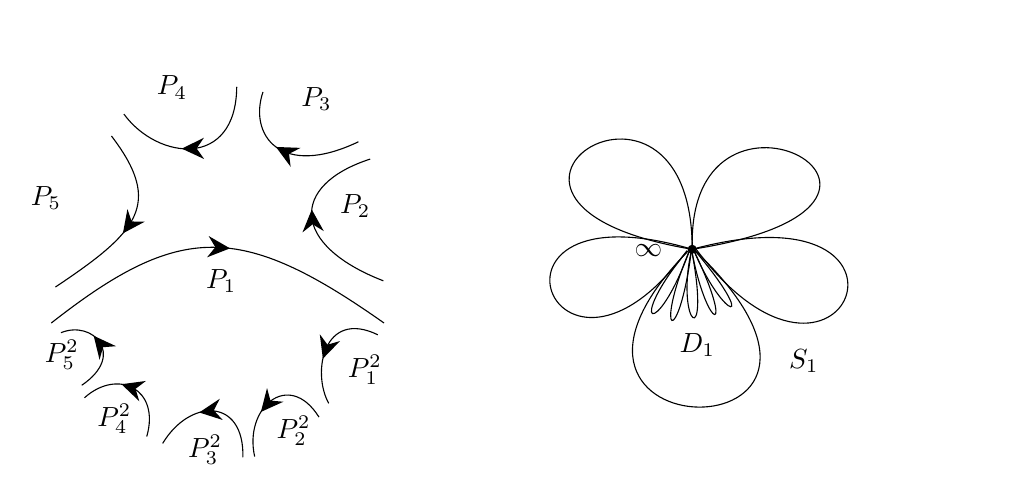
\begin{tikzpicture}[x=0.75pt,y=0.75pt,yscale=-1,xscale=1]
%uncomment if require: \path (0,300); %set diagram left start at 0, and has height of 300

%Curve Lines [id:da8105529734511654] 
\draw    (108,57.17) .. controls (124.33,79.5) and (162.07,83.64) .. (162.35,44) ;
\draw [shift={(135.91,73.82)}, rotate = 359.3] [fill={rgb, 255:red, 0; green, 0; blue, 0 }  ][line width=0.08]  [draw opacity=0] (10.72,-5.15) -- (0,0) -- (10.72,5.15) -- (7.12,0) -- cycle    ;
%Curve Lines [id:da5656492723103168] 
\draw    (226.67,78.83) .. controls (187.67,91.5) and (188.33,120.17) .. (233,137.5) ;
\draw [shift={(198.51,103.16)}, rotate = 86.49] [fill={rgb, 255:red, 0; green, 0; blue, 0 }  ][line width=0.08]  [draw opacity=0] (10.72,-5.15) -- (0,0) -- (10.72,5.15) -- (7.12,0) -- cycle    ;
%Curve Lines [id:da13626418538311813] 
\draw    (233.33,157.83) .. controls (164.33,109.17) and (135,109.17) .. (73,157.83) ;
\draw [shift={(159.13,121.86)}, rotate = 184.37] [fill={rgb, 255:red, 0; green, 0; blue, 0 }  ][line width=0.08]  [draw opacity=0] (10.72,-5.15) -- (0,0) -- (10.72,5.15) -- (7.12,0) -- cycle    ;
%Curve Lines [id:da4850842944262794] 
\draw    (126.67,215.83) .. controls (139.67,194.17) and (166,193.5) .. (165.33,222.5) ;
\draw [shift={(144.27,200.92)}, rotate = 352.09] [fill={rgb, 255:red, 0; green, 0; blue, 0 }  ][line width=0.08]  [draw opacity=0] (10.72,-5.15) -- (0,0) -- (10.72,5.15) -- (7.12,0) -- cycle    ;
%Curve Lines [id:da6830177286463675] 
\draw    (206.67,196.5) .. controls (198.33,181.5) and (204.33,150.83) .. (230.33,163.5) ;
\draw [shift={(203.85,175.03)}, rotate = 288.5] [fill={rgb, 255:red, 0; green, 0; blue, 0 }  ][line width=0.08]  [draw opacity=0] (10.72,-5.15) -- (0,0) -- (10.72,5.15) -- (7.12,0) -- cycle    ;
%Curve Lines [id:da8979306236335514] 
\draw    (171,222.17) .. controls (165.67,198.83) and (187.33,179.83) .. (202,203.17) ;
\draw [shift={(174.01,200.66)}, rotate = 310] [fill={rgb, 255:red, 0; green, 0; blue, 0 }  ][line width=0.08]  [draw opacity=0] (10.72,-5.15) -- (0,0) -- (10.72,5.15) -- (7.12,0) -- cycle    ;
%Shape: Circle [id:dp28811964079698127] 
\draw  [fill={rgb, 255:red, 0; green, 0; blue, 0 }  ,fill opacity=1 ] (379.9,122.3) .. controls (379.9,121.25) and (380.75,120.4) .. (381.8,120.4) .. controls (382.85,120.4) and (383.7,121.25) .. (383.7,122.3) .. controls (383.7,123.35) and (382.85,124.2) .. (381.8,124.2) .. controls (380.75,124.2) and (379.9,123.35) .. (379.9,122.3) -- cycle ;
%Curve Lines [id:da9630686419392767] 
\draw    (382.79,122.56) .. controls (490.56,225) and (281,222.33) .. (380.79,122.19) ;
%Curve Lines [id:da6952983011098728] 
\draw    (381.8,122.3) .. controls (520.87,100.6) and (380.47,25) .. (381.8,120.4) ;
%Curve Lines [id:da414714992696418] 
\draw    (381.8,120.4) .. controls (380.07,15.8) and (249.27,100.2) .. (381.8,122.3) ;
%Curve Lines [id:da63508389820832] 
\draw    (380.29,123.44) .. controls (364.42,167.06) and (349.66,159.26) .. (378.79,123.81) ;
%Curve Lines [id:da22495593911989342] 
\draw    (381.8,124.2) .. controls (389.29,162.69) and (402.79,164.81) .. (382.79,123.31) ;
%Curve Lines [id:da16912708964122225] 
\draw    (382.79,123.31) .. controls (397.36,157.62) and (414.9,160.38) .. (382.79,122.56) ;
%Curve Lines [id:da7915056796916238] 
\draw    (175,46.5) .. controls (168,67.17) and (183.33,88.5) .. (221,70.5) ;
\draw [shift={(181.25,73)}, rotate = 27.81] [fill={rgb, 255:red, 0; green, 0; blue, 0 }  ][line width=0.08]  [draw opacity=0] (10.72,-5.15) -- (0,0) -- (10.72,5.15) -- (7.12,0) -- cycle    ;
%Curve Lines [id:da06174169363528992] 
\draw    (102,67.73) .. controls (127.33,100.83) and (114.33,114.17) .. (75,140.5) ;
\draw [shift={(107.51,114.63)}, rotate = 306.28] [fill={rgb, 255:red, 0; green, 0; blue, 0 }  ][line width=0.08]  [draw opacity=0] (10.72,-5.15) -- (0,0) -- (10.72,5.15) -- (7.12,0) -- cycle    ;
%Curve Lines [id:da6193229855841036] 
\draw    (89,193.83) .. controls (105,179.5) and (125.67,189.5) .. (119,212.5) ;
\draw [shift={(106.83,187.31)}, rotate = 18.1] [fill={rgb, 255:red, 0; green, 0; blue, 0 }  ][line width=0.08]  [draw opacity=0] (10.72,-5.15) -- (0,0) -- (10.72,5.15) -- (7.12,0) -- cycle    ;
%Curve Lines [id:da06319156006210047] 
\draw    (77.67,162.5) .. controls (93,156.17) and (109.33,173.17) .. (87.67,187.83) ;
\draw [shift={(93.44,163.98)}, rotate = 50.62] [fill={rgb, 255:red, 0; green, 0; blue, 0 }  ][line width=0.08]  [draw opacity=0] (10.72,-5.15) -- (0,0) -- (10.72,5.15) -- (7.12,0) -- cycle    ;
%Curve Lines [id:da600082967290146] 
\draw    (383.7,122.3) .. controls (455.25,217.04) and (504.87,89) .. (381.8,122.3) ;
%Curve Lines [id:da0010692790397923702] 
\draw    (379.29,122.94) .. controls (315.27,210.2) and (268.87,89) .. (381.8,122.3) ;
%Curve Lines [id:da9686102352343344] 
\draw    (381.17,124.06) .. controls (373.92,158.69) and (390.67,172.31) .. (381.8,124.2) ;
%Curve Lines [id:da07465915682499946] 
\draw    (380.29,123.44) .. controls (363.04,164.31) and (375.17,171.19) .. (381.42,122.94) ;

% Text Node
\draw (146.29,130.84) node [anchor=north west][inner sep=0.75pt]    {$P_{1}$};
% Text Node
\draw (210.95,94.51) node [anchor=north west][inner sep=0.75pt]    {$P_{2}$};
% Text Node
\draw (192.24,42.92) node [anchor=north west][inner sep=0.75pt]    {$P_{3}$};
% Text Node
\draw (214.62,171.84) node [anchor=north west][inner sep=0.75pt]    {$P_{1}^{2}$};
% Text Node
\draw (180.29,201.51) node [anchor=north west][inner sep=0.75pt]    {$P_{2}^{2}$};
% Text Node
\draw (137.62,210.51) node [anchor=north west][inner sep=0.75pt]    {$P_{3}^{2}$};
% Text Node
\draw (352.81,118.66) node [anchor=north west][inner sep=0.75pt]    {$\infty $};
% Text Node
\draw (374.46,161.54) node [anchor=north west][inner sep=0.75pt]    {$D_{1}$};
% Text Node
\draw (427.23,169.33) node [anchor=north west][inner sep=0.75pt]    {$S_{1}$};
% Text Node
\draw (122.57,37.59) node [anchor=north west][inner sep=0.75pt]    {$P_{4}$};
% Text Node
\draw (61.9,90.92) node [anchor=north west][inner sep=0.75pt]    {$P_{5}$};
% Text Node
\draw (93.95,195.51) node [anchor=north west][inner sep=0.75pt]    {$P_{4}^{2}$};
% Text Node
\draw (68.62,164.84) node [anchor=north west][inner sep=0.75pt]    {$P_{5}^{2}$};


\end{tikzpicture}
\caption{$f_2:S^2 \rightarrow S^2$.}
\end{center}
\end{figure}


We now define $f_2\in \H$ such that $f_{2|S_1}=f_{1|S_1}$ and $f_{2|D_1}$ verifies $o( f_{2|D_1})=[a_2(n)]$. The construction is made in an analogous way by adding new planes $P^2_i$ and using the lower semi-plane of $P_1$. Figure \ref{disf2} represents the construction of $f_2$. 



We choose one of the new planes and call $D_2$ to the region associated to its lower half-plane. We call $S_2$ to the closure of the complement of $D_2$ and observe that dynamics created so far lay entirely in $S_2$. In particular, 
\[o(f_{2|S_2})=o(f_2)=\sup\{o(f_{2|S_1}), o(f_{2|D_1})\}=\sup \{[a_1(n)],[a_2(n)]\}= [a_2(n)].\]

Inductively, we define a family of regions  $D_k$ and $S_k=\overline{D_k^c}$ where $D_k$ is a disk, contains $\infty$ in its border, $D_{k+1}\subset D_k$, and we may also ask that $diam(D_k)\to 0$. By induction, we also have a family of maps $f_k\in \H$ such that:
\begin{itemize}
\item  $f_k(S_i)=S_i$ for all $i\leq k$. 
\item  $f_{k+1|S_k}= f_{k|S_k}$.
\item  $o(f_k)= o(f_{k|S_k})=[a_k(n)]$. 
\end{itemize}

This family of dynamical systems in $\H$ define a unique map $f\in \H$ with $f(x)=f_k(x)$ if $x\in S_k$.

Let us check if $o(f)=\sup(\Gamma)$. We first observe that
\[o(f)\geq o(f_{|S_k})= o(f_{k|S_k})=[a_k(n)], \]
thus, $o(f)\geq\sup (\Gamma)$. To see the other inequality, we chose $\e>0$ and $k$ such that $diam(D_k)\leq \e/2$. Since $f(D_k)= D_k$, for any $x_k\in D_k$, the dynamical ball $B(x_k,n,\e)$ contains $D_k$ for every $n$. If $G_n$ is an $(n,\e)$ generator set of $f_{|S_k}$ with 
$g_{f_{|S_k},\e}(n) =   \#G_n$, then $G_n\cup \{x_k\}$ is an $(n,\e)$-generator set of $f$. Therefore, 
$g_{f,\e}(n)\leq g_{f_{|S_k},\e}(n) +1 $ and then 
\[ [g_{f,\e}(n)]\leq [g_{f_{|S_k},\e}(n)]\leq o(f_{|S_k} ) = [a_k(n)]\leq \sup (\Gamma).\]
From this, we conclude  that $o(f)\leq \sup (\Gamma)$. This proves $o(f)=\sup (\Gamma)$ and finishes the proof of theorem \ref{teoFlex}.

